\documentclass[a4paper,12pt]{scrartcl}

\usepackage[utf8]{inputenc}
\usepackage[ngerman]{babel}
\usepackage{scrpage2}\pagestyle{scrheadings}
\usepackage{graphicx}
\usepackage{pgfplots}
\usepackage{multicol}
\usepackage{tikz}
\usepackage{amssymb}
\usepackage{amsmath}
\usepackage{ulem}

\ihead{Aufgabenblatt 3}
\ohead{\today}
\chead{Gruppe Dammer, Teuteberg, Wilhelm}
\pagestyle{scrheadings}

\begin{document}


\section{Konzeptioneller Entwurf}

\centerline{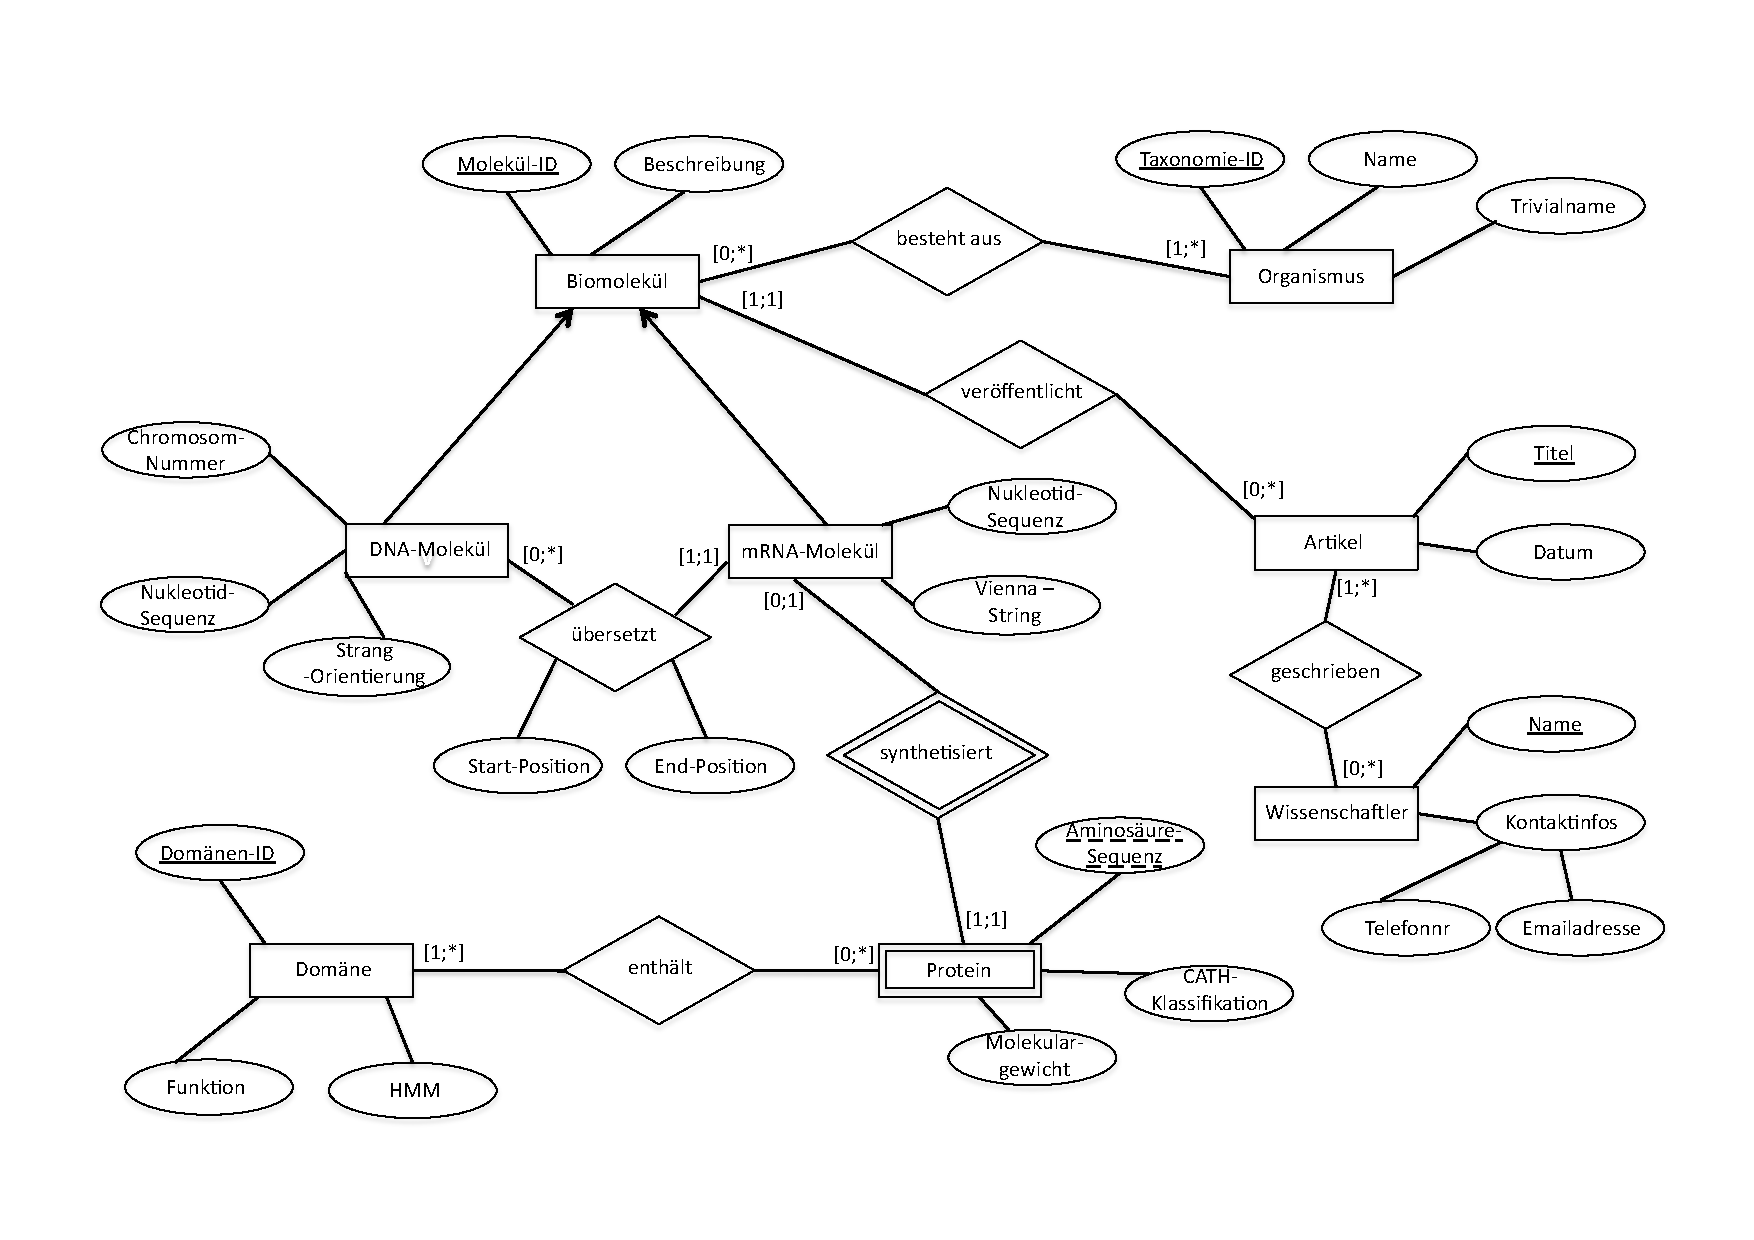
\includegraphics[scale=0.5]{A1_ERM.pdf}} \par 

\section{Logischer Entwurf}

Film(\underline{Titel}, \dashuline{Name $\rightarrow$ Regisseur.Name}, Zusammenfassung, 1.Drehtag, letzter Drehtag)

Charakter(\underline{CID}, Name, Charakterbeschreibung)

Genre(\underline{Name})

Regisseur(\underline{Name}, \dashuline{Name $\rightarrow$ Genre.Name}) oder Regisseur(\underline{\dashuline{Name $\rightarrow$ Person.Name}}, \dashuline{Name $\rightarrow$ Genre.Name})

Schauspieler(\underline{Name}) oder Schauspieler(\underline{\dashuline{Name $\rightarrow$ Person.Name}})

Person(\underline{Name}, DOB,Geschlecht)

Markenzeichen(\underline{\dashuline{Name $\rightarrow$ Schauspieler.Name}, Zeichen})

geh\"ort zu(\underline{\dashuline{Titel $\rightarrow$ Film.Titel}, \dashuline{Name $\rightarrow$ Genre.Name}})

spielt(\underline{\dashuline{Name $\rightarrow$ Schauspieler.Name}, \dashuline{CID $\rightarrow$ Charakter.CID}, \dashuline{Titel $\rightarrow$ Film.Titel}}, Drehbeginn, Drehende, Gage)



\section{Relationale Algebra und SQL}
\begin{enumerate}
  \item[a)]
  \begin{enumerate}
   \item [i)] Finde alle (Namen) Rennfahrer, die 1 Platz in ``Malaysia GP'' genommen haben.
   \item[ii)] Finde alle Rennfahrer, die in Rennstall mit Budget kleiner 350 teilgenommen haben.
   \item[iii)] Finde alle Teams (Rennstall), deren Rennfahrern ein Paltz in ``Australian GP" genommen haben.
  \end{enumerate}
  \item[b)]
  \begin{enumerate}
  \item[i)] $\pi_{Rennstall.Name} (\sigma_{Geburt>=1985}(Rennfahrer \Join Renntall))
  \\ \rightarrow \text{\{(Red Bull, McLaren)\}}$
     
  \item[ii)] $\pi_{Voraname,Nachname,Geburt} ((\sigma_{Rennstall=31}Rennfahrer) \Join \sigma_{OID=4}Platzierung) 
   \\ \rightarrow \text{\{(Lewis Hamilton 1985-01-07), (Jenson Button 1980-01-19)\}}$
   
   \item[iii)] $(Rennfahrer)-(\pi_{RID,Vorname,Nachname,Geburt,Wohnort,Rennstall}(Rennfahrer \Join Platzierung)
   \\ \rightarrow \text{\{(44 Kimi R\"aikk\"onen 1979-10-17 Espoo(Finnland) 34) \}}$
   
   \item[iv)] $\pi_{Vorname,Nachname}(\sigma_{Rennstall=\pi_{Rennstall}(\sigma_{RID=20}Rennfahrer)})
   \\ \rightarrow \text{\{(Lewis Hamilton)\}}$
  \end{enumerate}
  \item[c)]
  \begin{enumerate}
   \item[i)] 
   \begin{verbatim}
    SELECT
      rf.Vorname, rf.Nachname, rf.Geburt
    FROM
      Rennfahrer rf,
      Platzierung pl,
    WHERE
      pl.OID = 4 AND
      rf.Rennstall = 31
   \end{verbatim}
   
   \item[ii)]
   \begin{verbatim}
    SELECT
      Vorname, Nachname
    FROM
      Rennfahrer
    WHERE
      Rennfahrer.Rennstall = 31 AND
      Rennfahrer.Vorname != "Button"
   \end{verbatim}
  \end{enumerate}
\end{enumerate}

\newpage

\section{Algebraische Optimierung}
\begin{enumerate}
 \item[a)]
 \begin{tikzpicture}[baseline]
 \draw (-3, -6) node (Rennfahrer) {$Rennfahrer$};
 \draw (0, -6) node (Platzierung) {$Platzierung$};
 \draw (3, -6) node (Rennort) {$Rennort$};
 \draw (-1, -5) node (j1) {$\Join$};
 \draw (0, -4) node (j2) {$\Join$};
 \draw (0, -3) node (s1) {$\sigma_{Platz<11}$};
 \draw (0, -2) node (s2) {$\sigma_{Name=''China GP''}$};
 \draw (0,-1) node (p1) {$\pi_{Wohnort}$};
 \draw (0,0) node (final) {};
 
 \draw (final) -- (p1);
 \draw (p1) -- (s2);
 \draw (s2) -- (s1);
 \draw (s1) -- (j2);
 \draw (j2) -- (j1);
 \draw (j2) -- (Rennort);
 \draw (j1) -- (Rennfahrer);
 \draw (j1) -- (Platzierung);
 \end{tikzpicture}
 \item[b)]
 \begin{tikzpicture}
 \draw (-2, -5) node (Rennfahrer) {$Rennfahrer$};
 \draw (1, -5) node (Platzierung) {$Platzierung$};
 \draw (4, -5) node (Rennort) {$Rennort$};
 \draw (4, -4) node (s2) {$\sigma_{Platz<11}$};
 \draw (1, -4) node (s1) {$\sigma_{Name=''China GP''}$};
 \draw (2, -3) node (j2) {$\Join$};
 \draw (0, -2) node (j1) {$\Join$};
 \draw (0, -1) node (p1) {$\pi_{Wohnort}$};
 \draw (0, 0) node (final) {};
 
 \draw (final) -- (p1);
 \draw (p1) -- (j1);
 \draw (j1) -- (j2);
 \draw (j1) -- (Rennfahrer);
 \draw (j2) -- (s1);
 \draw (j2) -- (s2);
 \draw (s1) -- (Platzierung);
 \draw (s2) -- (Rennort);
 \end{tikzpicture}
 
 Ausdruck b) hat den höchsten Optimierungsgrad: Nach der Optimierungsheuristik I, 
 werden Selektionen möglichst früh ausgeführt, nach II werden die Projektionen möglichst früh  ausgeführt und nach III 
 werden Operatoren Selektion und Projektion verknüpft. In Ausdruck a) werden erst die Relationen verknüpft und dann 
 die Selektionen und Projektionen durchgeführt, das ist nicht effizient. \\
\end{enumerate}

\end{document}